\documentclass[11pt]{article}

\usepackage[margin=0.85in]{geometry}
\usepackage{amsmath,amssymb,bm,mathtools}
\usepackage{booktabs,longtable,tabularx,array}
\usepackage{graphicx,subcaption,float,placeins}
\usepackage{enumitem}
\usepackage{microtype}
\usepackage{xcolor}
\usepackage{hyperref}

\hypersetup{
  colorlinks=true,
  linkcolor=blue!45!black,
  urlcolor=blue!55!black,
}

\newcommand{\G}{\mathcal{G}}
\newcommand{\Gref}{G_{6}}
\newcommand{\Gmodel}{G_{\theta}}
\newcommand{\norm}[1]{\left\lVert #1\right\rVert}
\newcommand{\inner}[2]{\left\langle #1,#2\right\rangle}
\newcommand{\dd}{\mathop{}\!\mathrm{d}}
\newcommand{\eref}{e_{\eta}}
\newcommand{\eshift}{e_{\eta,\mathrm{shift}}}
\allowdisplaybreaks

\title{Evaluation of a Learned Dirichlet--Neumann Operator\\
and Experiments Conducted 9--16 July 2026}
\author{Internal mathematical report}
\date{Revised 16 July 2026\\Data cutoff: 04:08 EDT}

\begin{document}
\maketitle

\begin{abstract}
We evaluate a learned Dirichlet--Neumann operator in long water-wave
calculations.  The learned and reference calculations use the same spatial
grid and the same two-stage Gauss--Legendre integrating-factor method.  They
differ in the evaluation of $q=G(\eta)\xi$: the reference uses a Craig--Sulem
expansion through order six, evaluated with eightfold Fourier padding, whereas
the learned calculation uses model C21.  The order-six calculation is a
numerical reference; it is not the exact solution of the continuum problem.

We attempted 2,560 rollouts, consisting of 256 newly generated initial
conditions from each of ten panels.  Fifty-two reference calculations were
excluded because the reference contained a nonfinite value or its relative
Hamiltonian drift exceeded $10^{-3}$.  Among the remaining 2,508 cases, no C21
rollout contained a nonfinite value in $\eta$, $\xi$, or $G_\theta(\eta)\xi$ at
any saved time.  The empirical median, 95th percentile, 99th percentile, and
maximum of the terminal relative elevation error were
$0.00563$, $0.1693$, $0.4854$, and $1.3262$.  Six cases had error above one.

Five of those six cases belong to the Tanaka initial-condition distribution.
For these five cases, one optimal periodic translation of the final predicted
surface removes 98.14--99.96\% of the squared elevation error.  The sixth is a
Benjamin--Feir case.  Its relative error decreases only from $1.1036$ to
$0.8422$ after translation because several important Fourier modes have
incorrect amplitudes and mutually inconsistent phase errors.

The report also explains why each experiment during 9--16 July was reasonable
before it was run.  Earlier models had small errors on reference states but a
bad response to perturbations away from those states.  This motivated exact
evaluation of $G_0+G_1$, a learned correction that begins at second order in
$\eta$, self-adjointness in $\xi$, and a loss based on the Hadamard shape
derivative.  These changes were made together in C16, after which no nonfinite
state was observed on the fixed 320-case test.  Because the changes were
bundled, this experiment does not identify which ingredient was individually
necessary.  Later losses aimed at Fourier modes or horizontal wave speed
improved average errors but did not improve every large-error case.  In two
diagnostic Tanaka calculations, none of the tested partial corrections to the
DNO error improved both cases.  Correcting the complete DNO error reproduced
the order-six calculation to approximately $2\times10^{-8}$.  C25 increases
the size of the learned correction while retaining the C20 loss.  It completed
two epochs before stopping during epoch 3 and has no rollout evaluation, so it
is not included in the rollout conclusions.
\end{abstract}

\tableofcontents
\newpage

\section{Question addressed by this report}

The project has two different numerical questions.

\begin{enumerate}[leftmargin=*]
  \item Does replacing the numerical Dirichlet--Neumann operator by the
  learned operator cause the time integration to produce NaN or Inf before
  the final time?

  \item Conditional on the rollout remaining finite, how accurately does the
  learned calculation reproduce the numerical reference?
\end{enumerate}

These questions must be kept separate.  An absence of NaNs is not a statement
that the terminal error is small.  Conversely, a large but finite phase error
does not imply that the time integrator has become unstable.

The principal empirical statement in this report is deliberately narrow:

\begin{quote}
C21 produced no nonfinite value on the 2,508 reference-valid cases in the new
test.  It nevertheless produced six finite terminal elevation errors above
one.
\end{quote}

The following sections define every object in this statement, give the
corresponding statistics, and describe the experiments that led to C21.

\section{Mathematical and numerical definitions}

\subsection{Water-wave variables and the Dirichlet--Neumann operator}

Let $x\in[0,2\pi)$ be periodic, let $\eta(x,t)$ be the free-surface elevation,
and let $\xi(x,t)$ be the velocity potential restricted to the free surface.
For a fluid of constant depth $h$, the Dirichlet--Neumann operator maps the
surface potential to the normal velocity of the surface.  We write
\begin{equation}
  q(\eta,\xi;h)=G(\eta;h)\xi.
  \label{eq:q-def}
\end{equation}
In Zakharov variables, with gravity $g=1$, the equations used by the code are
\begin{align}
  \eta_t
  &=q,                                                    \label{eq:zak-eta}\\
  \xi_t
  &=-\eta-\frac12\xi_x^2
    +\frac12\frac{(q+\eta_x\xi_x)^2}{1+\eta_x^2}.        \label{eq:zak-xi}
\end{align}
Thus an error in $q$ enters both equations: it is the complete right-hand side
of \eqref{eq:zak-eta} and appears quadratically in \eqref{eq:zak-xi}.

For the flat surface, the Fourier symbol of the DNO is
\begin{equation}
  \widehat{G_0(h)\xi}_k=|k|\tanh(h|k|)\widehat\xi_k.
  \label{eq:g0}
\end{equation}
The first shape-dependent Craig--Sulem term is evaluated from
\begin{equation}
  G_1(\eta;h)\xi
  =-G_0(h)\bigl(\eta G_0(h)\xi\bigr)
   -\partial_x\bigl(\eta\,\partial_x\xi\bigr).
  \label{eq:g1}
\end{equation}
The cancellation between the two terms in \eqref{eq:g1} is important for
same-sign high-frequency interactions.  Asking a neural network to learn the
two large terms separately can destroy this cancellation even when its mean
value error is small.

\subsection{The numerical reference and the learned calculation}

All reported calculations use $N_x=1024$ equispaced points on $[0,2\pi)$.
The numerical reference evaluates
\begin{equation}
  \Gref(\eta;h)\xi=\sum_{m=0}^{6}G_m(\eta;h)\xi
  \label{eq:g6}
\end{equation}
with eightfold Fourier padding for products.  The nonlinear terms in
\eqref{eq:zak-xi} are evaluated on a grid with twice as many points and then
truncated back to the base grid.  We call this calculation the
\emph{order-six numerical reference}.  The notation $G_6$ refers to the
truncated Craig--Sulem series in \eqref{eq:g6}; it does not assert equality
with the continuum DNO.

Models C20, C21, and C25 have the form
\begin{equation}
  \Gmodel(\eta;h)\xi
  =G_0(h)\xi+G_1(\eta;h)\xi+R_\theta(\eta,\xi,h),
  \qquad R_\theta=O(\eta^2).
  \label{eq:model}
\end{equation}
The terms $G_0$ and $G_1$ are evaluated from their formulas, without an
additional learned cutoff.  The network approximates the remainder beginning
with $G_2$.

Each learned block is a sum of multiplier sandwiches of the form
\begin{equation}
  R_{b}(\eta,\xi,h)
  =\sum_{j=1}^{r}M_{b,j}(h,D)
       \left[\phi_{b,j}(\eta,h)\,M_{b,j}(h,D)\xi\right].
  \label{eq:block}
\end{equation}
The same real Fourier multiplier $M_{b,j}$ is used on the two sides of the
pointwise multiplication.  Consequently \eqref{eq:block} is self-adjoint as
an operator in $\xi$ for fixed $\eta$ and $h$.  The feature network has no
bias, hence is $O(\eta)$ near $\eta=0$; its final lift is
$f\mapsto f\tanh f=O(f^2)$.  Therefore the learned correction in
\eqref{eq:model} is $O(\eta^2)$ by construction.  The sum over blocks and
branches is divided by the square root of their number.  This normalization
controls the size of a parameter update as the number of branches is changed;
it does not reduce the set of functions representable after training.

\subsection{Time integration}

The linear system containing $G_0$ is solved exactly in Fourier space inside
an integrating-factor formulation.  The remaining system is advanced by the
two-stage Gauss--Legendre Runge--Kutta method.  If $v_n$ is the integrating-
factor state and $F$ denotes its nonlinear right-hand side, the stage
equations are
\begin{align}
  V_1 &=v_n+\Delta t\,(a_{11}F(V_1)+a_{12}F(V_2)),\\
  V_2 &=v_n+\Delta t\,(a_{21}F(V_1)+a_{22}F(V_2)),\\
  v_{n+1}&=v_n+\frac{\Delta t}{2}\bigl(F(V_1)+F(V_2)\bigr),
  \label{eq:gl2}
\end{align}
where
\begin{equation}
  a_{11}=a_{22}=\frac14,
  \qquad
  a_{12}=\frac14-\frac{\sqrt3}{6},
  \qquad
  a_{21}=\frac14+\frac{\sqrt3}{6}.
\end{equation}
Four Picard iterations are used to approximate the coupled stages.  The inner
step is $\Delta t=0.01$ in every panel.  Long Tanaka and Benjamin--Feir
calculations are saved every $0.8$ time units and end at $T=200$; the other
panels are saved every $0.08$ and end at $T=20$.  The nonlinear right-hand
side and the updated state are projected onto $|k|\leq128$, corresponding to
the configured filter fraction $0.25$.  No additional runtime damping,
cutoff, or fallback was enabled in the C21 evaluation reported here.

The order-six and learned rollouts use the same numerical choices.  Their
intended difference is the map used to compute $q$.  The reference stage
arithmetic is float64.  The C21 network evaluates $q$ in float32 and returns it
to the float64 integration harness.  Both completed trajectories are cast to
float32 before archival and before the validity and error calculations below.
Thus all reported error statistics include this mixed-precision implementation
of the learned operator and are computed from float32 archives.

\subsection{An exact decomposition of numerical rollout error}

Let $z=(\eta,\xi)$.  Denote one complete filtered GL2 step using $G_6$ by
$\Phi_6$ and the corresponding step using $G_\theta$ by $\Phi_\theta$:
\begin{equation}
  z_{n+1}^{6}=\Phi_6(z_n^6),
  \qquad
  z_{n+1}^{\theta}=\Phi_\theta(z_n^\theta).
\end{equation}
Adding and subtracting $\Phi_6(z_n^\theta)$ gives the exact identity
\begin{equation}
\begin{split}
 z_{n+1}^{\theta}-z_{n+1}^{6}
 ={}&\underbrace{\Phi_\theta(z_n^\theta)-\Phi_6(z_n^\theta)}_{A_n:
 \text{ difference caused by the learned DNO at the current model state}}\\
 &+\underbrace{\Phi_6(z_n^\theta)-\Phi_6(z_n^6)}_{B_n:
 \text{ propagation of state error already present}}.
\end{split}
\label{eq:map-split}
\end{equation}
No linearization is used in \eqref{eq:map-split}.  The identity explains the
logic of the experiments in this report.  Pointwise supervised training tries
to make $A_n$ small on states drawn from the reference data.  Rollouts also
require $A_n$ to remain controlled at states generated by the imperfect model.
Even when $A_n$ is small, the nonlinear reference map can amplify accumulated
state error through $B_n$.  Conversely, observing growth in $B_n$ does not
show that the numerical reference is wrong: $B_n$ is the response of the same
reference map to two different states.

\section{Evaluation population and error measures}

\subsection{Initial-condition panels}

The evaluation contains ten named panels, with 256 independently generated
initial conditions in each panel.  The labels \emph{g0}, \emph{g1}, and
\emph{modal} do not denote different equations or different DNO orders in
this evaluation.  They denote independent random-number streams from the same
Tanaka or Benjamin--Feir distribution.  Table~\ref{tab:ic-families} gives the
actual distinctions.

\begin{table}[htbp]
\centering
\small
\begin{tabularx}{\textwidth}{p{.17\textwidth}X p{.18\textwidth}}
\toprule
Panels & Construction of one initial condition & Horizon \\
\midrule
Tanaka g0, g1
& Sum of one to three separated solitary-wave profiles.  Total steepness is
drawn between .10 and .35.  Dirichlet weights are clamped at .05 before a
final renormalization to the sampled total; consequently .05 is not a strict
lower bound on the final steepness of each crest.  Depth is log-uniform on
$[.01,.30]$.
& $T=200$ \\

BF g0, g1, modal
& A carrier with wavenumber 4--20 and steepness .05--.13, plus two sidebands
offset by 2--4 modes with relative amplitudes .05--.20 and independent phases.
Second-order corrections are included.  Depth is log-uniform on $[.5,4]$.
& $T=200$ \\

Linear
& A nominal single-mode wave with mode 1--20, random direction and phase, and
steepness .005--.15.  The reference rollout is nevertheless the nonlinear
order-six calculation.
& $T=20$ \\

Random sea, deep
& Gaussian spectrum with significant height .005--.03, peak wavenumber 2--12,
bandwidth 1.5--5, independent phases, and log-uniform depth $[5,25]$.
& $T=20$ \\

Random sea, finite depth
& The same spectral construction with log-uniform depth $[.1,1.5]$.
& $T=20$ \\

Stokes, deep
& A random-phase fifth-order Stokes profile with base mode 1--20, steepness at
most .15, and depth in $[4,50]$ subject to the generator's $kh$ constraint.
& $T=20$ \\

Stokes, finite depth
& A random-phase fifth-order Stokes profile with base mode 14--26, steepness at
most .15, and depth in $[.02,1.5]$ subject to the generator's $kh$ constraint.
& $T=20$ \\
\bottomrule
\end{tabularx}
\caption{Initial-condition distributions used in the new evaluation.  The
three Tanaka/BF replicate labels are retained because the corresponding
training sources were stored separately; physically, each replicate uses the
same distribution as the other panels in its group.}
\label{tab:ic-families}
\end{table}

The panels were generated from recorded parameters and the master seed
20,260,715.  Each panel uses a separate NumPy \texttt{SeedSequence} stream
that is absent from the training metadata.  The builder checks hashes of the
new initial states and rejects duplicates among the new panels.  No archived
training trajectory was selected.  The builder does not, however, compare
the hash of every new state against every state in the training archive.
Disjointness is therefore established by independent generation and its saved
generation record, not by an exhaustive cross-hash.  The construction also does not
establish generalization to distributions absent from
Table~\ref{tab:ic-families}.

\subsection{Reference validity and model finiteness}

For a saved numerical trajectory define the discrete Hamiltonian
\begin{equation}
  H_j=\frac{\Delta x}{2}\sum_{m=0}^{N_x-1}
  \left(\xi_{j,m}q_{j,m}+\eta_{j,m}^2\right).
  \label{eq:discrete-H}
\end{equation}
A reference trajectory is called \emph{valid} if
\begin{enumerate}[leftmargin=*]
  \item all saved values of $\eta^6$, $\xi^6$, and $q^6$ are finite; and
  \item $\max_j |H_j-H_0|/(|H_0|+10^{-12})\leq10^{-3}$.
\end{enumerate}
The threshold was fixed in the evaluation code before the statistics were
computed.  A learned rollout is called \emph{nonfinite} if any saved value of
$\eta^\theta$, $\xi^\theta$, or $q^\theta$ is NaN or Inf.  Notice that this
definition examines saved frames.  It does not separately inspect every
intermediate floating-point operation inside a completed GL2 step.

The complete validity table is
\begin{table}[htbp]
\centering
\begin{tabular}{lrrr}
\toprule
Order-six reference & C21 finite & C21 nonfinite & Total \\
\midrule
Valid   & 2508 & 0 & 2508 \\
Invalid & 49   & 3 & 52 \\
\midrule
Total   & 2557 & 3 & 2560 \\
\bottomrule
\end{tabular}
\caption{Reference validity and C21 finiteness.  Accuracy statistics below use
only the 2,508 reference-valid cases.  The three nonfinite C21 calculations on
reference-invalid cases are reported here but cannot be used to score
accuracy against a valid reference.}
\label{tab:validity}
\end{table}
Among the 52 excluded references, 24 contain a nonfinite archived field and 28
additional finite references exceed the Hamiltonian-drift threshold.  The
three nonfinite C21 calculations in the second row occur in one linear-panel
case and two finite-depth random-sea cases.

\subsection{Raw and translation-aligned errors}

The primary terminal error is
\begin{equation}
  \eref(T)=
  \frac{\norm{\eta^\theta(\cdot,T)-\eta^6(\cdot,T)}_{\ell^2}}
       {\norm{\eta^6(\cdot,T)}_{\ell^2}}.
  \label{eq:raw-error}
\end{equation}
To measure how much of this discrepancy is caused only by horizontal wave
position, define
\begin{equation}
  \eshift(T)=\min_{s\in[0,2\pi)}
  \frac{\norm{\eta^\theta(\cdot-s,T)-\eta^6(\cdot,T)}_{\ell^2}}
       {\norm{\eta^6(\cdot,T)}_{\ell^2}}.
  \label{eq:shift-error}
\end{equation}
The shift is applied to the predicted final elevation only.  It is not used
during the rollout and it is not an acceptance metric.  It answers the more
limited question: how small would the terminal elevation error be if one were
allowed to correct a single periodic translation after the calculation?

The reported fraction of squared elevation error removed by this translation
is
\begin{equation}
  r_{\mathrm{shift}}
  =1-\left(\frac{\eshift(T)}{\eref(T)}\right)^2.
  \label{eq:rshift}
\end{equation}
The numerical approximation to the minimization in \eqref{eq:shift-error}
begins from the eight largest peaks of the discrete circular correlation and
refines each candidate by continuous Fourier translation within one grid
cell.  The smallest resulting value is retained.  This is a high-accuracy
search over the observed correlation peaks, not a proof that the global
continuous minimizer has been found for every profile.

All quantiles below are empirical quantiles of the finite values on the 2,508
reference-valid cases, using NumPy's linear interpolation convention.  They
are conditional on the deliberately constructed mixture of panels in
Table~\ref{tab:ic-families}.

\section{C21 results on the new initial conditions}

\subsection{Nonfinite events}

No C21 trajectory was nonfinite among the 2,508 reference-valid cases.  If one
models these cases as independent Bernoulli draws from exactly the same
mixture of initial-condition distributions, the one-sided Clopper--Pearson
95\% upper confidence bound after zero events in $n=2508$ trials is
\begin{equation}
  p_{\mathrm{upper}}=1-0.05^{1/2508}=1.194\times10^{-3}.
  \label{eq:zero-upper}
\end{equation}
This calculation does not prove that the event probability is zero.  It also
depends on treating the sampled initial conditions as independent draws and
does not apply to longer horizons or to a different family mixture.

\subsection{Pooled empirical errors}

Table~\ref{tab:pooled} reports all 2,508 valid cases as one sample.  Half of
the cases have raw terminal error below $0.00563$, 95\% have error below
$0.1693$, and the largest error is $1.3262$.  There are 83 errors above
$0.25$, 23 above $0.50$, 11 above $0.75$, and 6 above $1$.

\begin{table}[htbp]
\centering
\small
\setlength{\tabcolsep}{4pt}
\begin{tabular}{lrrrrrrrrr}
\toprule
Error & $n$ & Mean & $q_{25}$ & $q_{50}$ & $q_{75}$ & $q_{90}$ & $q_{95}$ & $q_{99}$ & Max \\
\midrule
Raw $\eref$
& 2508 & .034908 & .001229 & .005634 & .020413 & .083930 & .169262 & .485363 & 1.326217 \\
After one shift $\eshift$
& 2508 & .014649 & .000631 & .003709 & .011708 & .032467 & .058772 & .207540 & .842246 \\
\bottomrule
\end{tabular}
\caption{Empirical terminal relative elevation errors for C21.  The first row
is the primary error \eqref{eq:raw-error}.  The second row applies the
diagnostic final-time translation in \eqref{eq:shift-error}.}
\label{tab:pooled}
\end{table}

\begin{table}[htbp]
\centering
\small
\begin{tabular}{lrrrrrrrr}
\toprule
& \multicolumn{2}{c}{Error $>.25$} & \multicolumn{2}{c}{Error $>.50$}
& \multicolumn{2}{c}{Error $>.75$} & \multicolumn{2}{c}{Error $>1$} \\
Error & Count & Rate & Count & Rate & Count & Rate & Count & Rate \\
\midrule
Raw $\eref$ & 83 & 3.309\% & 23 & .917\% & 11 & .439\% & 6 & .239\% \\
After one shift $\eshift$ & 17 & .678\% & 5 & .199\% & 1 & .040\% & 0 & 0 \\
\bottomrule
\end{tabular}
\caption{Strict threshold counts on the same 2,508 cases.  The difference
between the rows measures the contribution of a single terminal horizontal
translation.  Seventeen cases still exceed .25 after this correction.}
\label{tab:thresholds}
\end{table}

\begin{figure}[htbp]
  \centering
  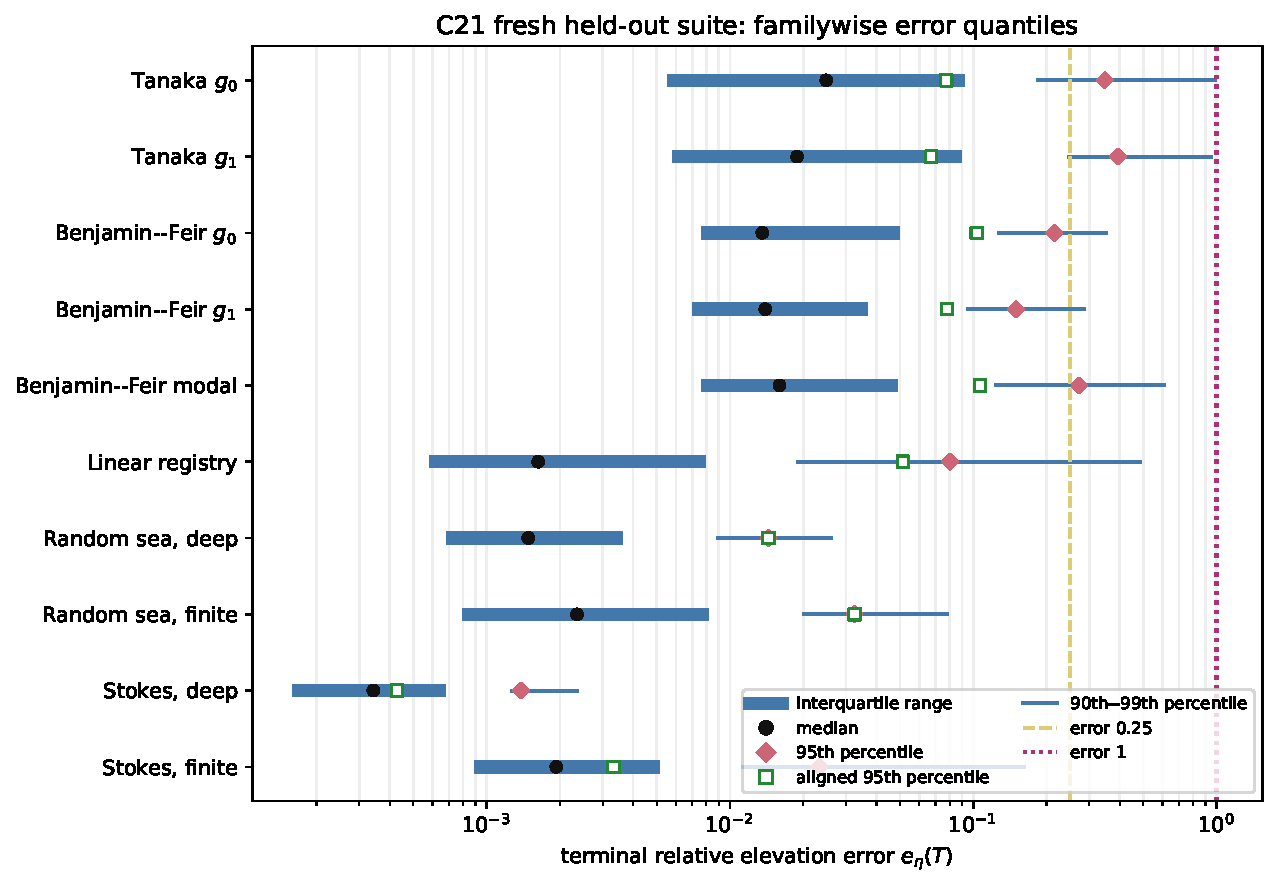
\includegraphics[width=\textwidth]{figures/weekly_results_20260716/c21_heldout_family_quantiles.pdf}
  \caption{Empirical error quantiles for each initial-condition panel.  The
  black circle is the median raw error.  The thick blue interval is the 25th
  to 75th percentile, the thin blue interval is the 90th to 99th percentile,
  and the red diamond is the 95th percentile.  The open green square is the
  95th percentile after the best final-time translation.}
  \label{fig:family-quantiles}
\end{figure}

\begin{figure}[htbp]
  \centering
  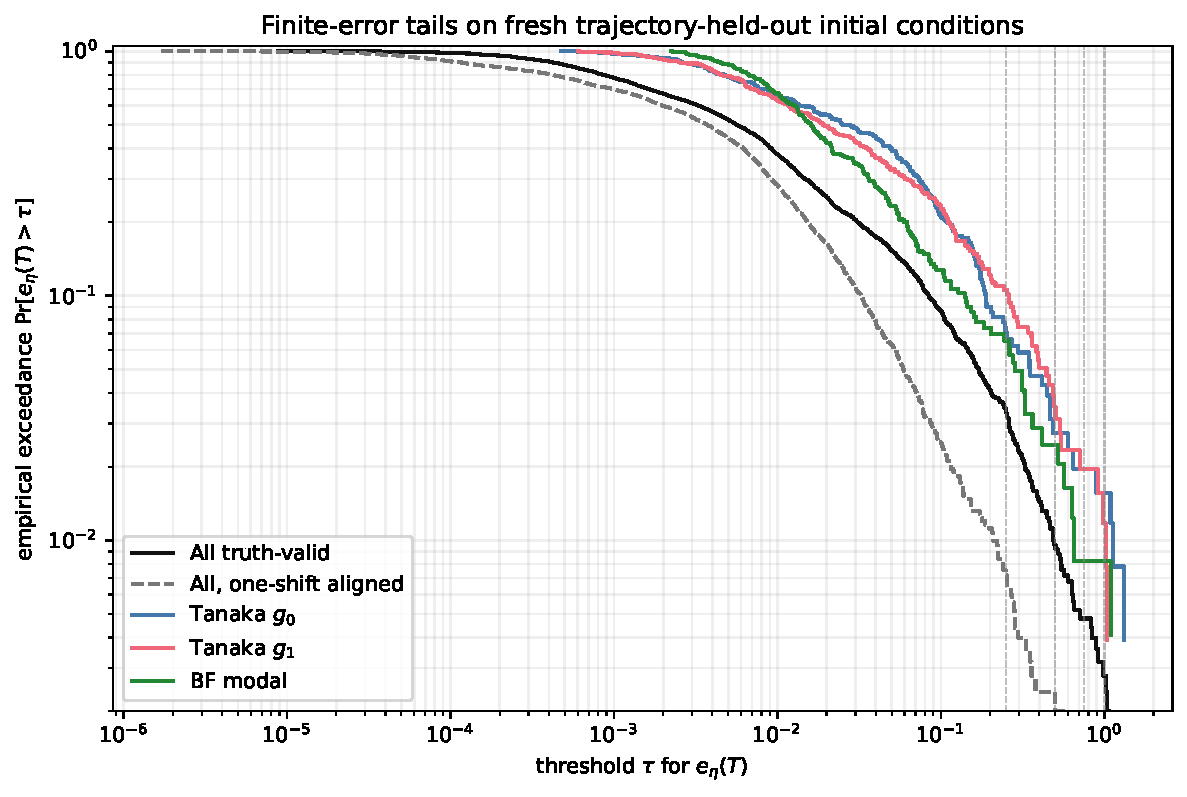
\includegraphics[width=.88\textwidth]{figures/weekly_results_20260716/c21_heldout_exceedance.pdf}
  \caption{For each error level $a$, the vertical coordinate is the empirical
  fraction of valid cases with terminal error larger than $a$.  Solid curves
  use the raw error.  Dashed curves use the error after one final-time
  translation.}
  \label{fig:exceedance}
\end{figure}

\FloatBarrier

% These final sections are defined here because they were assembled before the
% detailed loss/history sections below.  They are emitted after the failure
% analysis, immediately before \end{document}.
\long\def\FinalSections{%
\section{C25: what changed and what has been measured}

The reference-assisted calculations in Table~\ref{tab:stage-corrections} did
not identify a tested partial correction that improved both cases.  Since the
complete DNO discrepancy corrected both, one plausible remaining hypothesis
is that the learned remainder in \eqref{eq:model} lacks either representational
or effective optimization capacity.  A larger model is worth testing only if
the exact $G_0+G_1$ terms, the $O(\eta^2)$ and self-adjoint construction, the
data, and the loss are held fixed.

C25 changes
\begin{equation}
 (\text{feature width},\text{branch rank},\text{multiplier hidden width},
 \text{blocks})
 =(512,256,128,8)
 \longrightarrow(640,320,160,8).
\end{equation}
The parameter count increases from 860,928 to 1,342,400, or 55.9\%.  C25 is
initialized from random parameters.  It retains the exact $G_0+G_1$ terms,
the $O(\eta^2)$ self-adjoint learned remainder, and exactly the C20 objective
in \eqref{eq:all-objectives}.  No analytic $G_m$ with $m\geq2$ is added.  The
$\gamma^2$ and finite-time losses are zero.

A 1\%-data smoke test completed all 59 batches with finite losses and evaluated
the Hadamard term on the expected four batches.  In the full-data run, the first two completed
epochs are reported in Table~\ref{tab:c25-training}.
\begin{table}[H]
\centering
\begin{tabular}{lrrrr}
\toprule
Epoch & Training loss & Validation loss & Validation $H^1$ & Validation mode loss \\
\midrule
1 & .0114936 & .00969421 & .00900150 & .000106919 \\
2 & .00932340 & .00874953 & .00829122 & .0000722955 \\
\bottomrule
\end{tabular}
\caption{Completed C25 training epochs available at the revision cutoff.  The
validation loss is defined by Table~\ref{tab:val-losses}.}
\label{tab:c25-training}
\end{table}
Every recorded scalar in these epochs is finite, and expected and observed
Hadamard batches are 373/373 in both.  The process stopped during epoch 3 after
2,357 of 5,964 training batches; the available log contains no completed epoch
3 or rollout evaluation.  Therefore Table~\ref{tab:c25-training} is an
optimization-status report, not evidence about long-time error or NaNs.

The capacity hypothesis is supported only if a completed C25 checkpoint is
evaluated using the same comparisons as C21.  The required sequence is:
\begin{enumerate}[leftmargin=*]
  \item complete training without a nonfinite loss or a disagreement in
  optimizer steps or sparse-loss counts between the two GPU copies;
  \item evaluate the fixed 64 Tanaka cases, reporting raw and shifted errors;
  \item if that comparison improves, evaluate the ten new 256-case panels;
  \item compare the nonfinite count, pooled and panelwise empirical quantiles,
  and all four threshold counts to Tables~\ref{tab:validity}--\ref{tab:family-errors}.
\end{enumerate}
Even a positive result would show only that this larger trained model performs
better.  It would not prove that the smaller architecture cannot represent an
equally accurate DNO, because optimization and initialization also differ.

\section{Conclusions and their limits}

The numerical evidence supports the following statements.

\begin{enumerate}[leftmargin=*,label=\textbf{\arabic*.}]
  \item \textbf{Observed finiteness.}  Among 2,508 cases for which the
  order-six numerical reference satisfies the stated validity test, C21 has no
  saved NaN or Inf in $\eta$, $\xi$, or $q$.  This is a finite-sample statement
  for the seven sampled initial-condition distributions and the stated time
  horizons.  It is not a stability theorem.

  \item \textbf{Finite accuracy.}  The empirical raw median and 95th
  percentile are $.00563$ and $.1693$.  Six cases have raw terminal error above
  one.  Therefore ``no observed NaNs'' must not be replaced by ``no failures''
  or ``uniformly accurate.''

  \item \textbf{Tanaka displacement.}  In five of the six cases above one, a
  numerically optimized final periodic translation removes 98.14--99.96\% of
  squared elevation error.  Their fitted shifts grow over time, and the
  integrated phase-rate discrepancy from $q=\eta_t$ agrees with the measured
  phase accumulation.  This supports gradual horizontal displacement as the
  main source of terminal error in those cases.  It does not show that every
  intermediate error lies in a single neutral eigenmode.

  \item \textbf{Benjamin--Feir error.}  In the remaining case above one, the
  best translation leaves error $.8422$.  Important Fourier modes have
  different amplitude ratios and phase shifts of different signs.  A single
  horizontal position coordinate cannot describe this case.

  \item \textbf{Earlier NaNs.}  Before C16, small DNO value error on reference
  states coexisted with order-one residuals in the Hadamard shape identity and
  a large response to off-trajectory perturbations.  Spectral damping and
  integration changes modified the terminal behavior but did not prevent the
  old failures.  The bundled C16 change---explicit $G_0+G_1$, an
  $O(\eta^2)$ self-adjoint remainder, randomized Hadamard consistency, and
  twofold dealiasing---was followed by no observed nonfinite state on the fixed
  suite.  Because the ingredients were bundled, their individual necessity is
  not established.

  \item \textbf{Projected phase losses.}  Translation-speed, localized, and
  $\gamma^2$ losses have a clear mathematical rationale and improve selected
  phase-dominated cases.  They do not bound the worst case: an update that
  improves case 27 can worsen case 24.  The reference-assisted corrections
  likewise show that none of the tested modal, local, or radial components
  improves both cases.

  \item \textbf{Complete reference correction.}  Adding the complete
  discrepancy $q_6(z)-q_\theta(z)$ at every GL2 stage makes two diagnostic
  rollouts agree with their order-six counterparts to about $2\times10^{-8}$.
  This verifies numerical consistency of the two code paths once the DNO
  discrepancy is removed.  It is not a continuum convergence result and is
  not a usable surrogate because it evaluates $G_6$.

  \item \textbf{C25.}  C25 asks whether a larger learned remainder performs
  better when the C20 equations and objective are unchanged.  Two completed
  epochs are finite, but no C25 rollout result exists at this cutoff.  No claim
  about the capacity hypothesis is presently justified.
\end{enumerate}

\appendix

\section{Chronological index of experiments, 9--16 July}

This appendix places the grouped argument in calendar order.  ``Did not meet
criterion'' means the measured result did not justify using that run as the
next checkpoint.  ``No result'' means the necessary evaluation was not
completed.

\begingroup
\setlength{\tabcolsep}{3pt}
\begin{longtable}{p{.08\textwidth}p{.10\textwidth}p{.23\textwidth}p{.27\textwidth}p{.23\textwidth}}
\caption{Experiment chronology.}
\label{tab:chronology}\\
\toprule
Date & Run & Controlled question & Measured result & Conclusion permitted by the result \\
\midrule
\endfirsthead
\toprule
Date & Run & Controlled question & Measured result & Conclusion permitted by the result \\
\midrule
\endhead

9 Jul & C8
& Does a broad GL2 stage-gain loss on modes 16--128 prevent the observed
spectral growth?
& Tanaka remained at 3 nonfinite cases out of 32; Tanaka and BF medians
increased.
& The tested broad stage penalty did not meet the finiteness or accuracy
criterion. \\

9 Jul & C9
& Does a 33-fold stronger soft penalty on high-frequency $q$ reduce the
measured dangerous output?
& The diagnostic was essentially unchanged; Tanaka retained 3/32 nonfinite
cases and BF errors increased.
& Increasing this soft penalty did not control the measured quantity. \\

9 Jul & C10
& Does matching the evaluation filter and targeting only modes 64--128 improve
the stage-gain experiment?
& Tanaka nonfinite count decreased from 3/32 to 2/32, but finite errors
increased and the target of zero was not reached.
& The diagnosed band participates in failure, but the tested loss is not a
sufficient remedy. \\

9 Jul & Data audit
& Are nonfinite labels, the old sign-change warning, or model-harvested states
corrupting training?
& Sampled base rows were finite.  The model-harvested pre-failure pack had
2,943 flagged rows out of 3,855.
& Do not use the model-harvested pack as reference data.  The sampled audit is
not an exhaustive proof of base-label correctness. \\

9 Jul & C13
& Can exact reference labels near selected difficult states improve C10?
& Training completed with finite loss; rollout evaluation was canceled.
& No rollout conclusion. \\

9 Jul & C14
& Does an architectural bound on high-frequency output rule out the old
failure?
& Best finite checkpoint had 3/32 nonfinite Tanaka trajectories and 6/32 under
the legacy divergence definition; training became nonfinite after epoch 25.
& The tested bound did not meet the criterion. \\

9 Jul & C15
& Was C14's poor result caused by using only one block?
& Interrupted before epoch 1; no checkpoint.
& No result. \\

9--11 Jul & C16
& Does the bundled DNO structure motivated by $G_1$ cancellation and the
Hadamard identity eliminate the observed nonfinite calculations?
& The clean fixed suite had 0/320 nonfinite model trajectories; two finite
Tanaka errors exceeded one.
& The bundle met the fixed-sample finiteness criterion.  Individual ingredients
are not isolated. \\

11 Jul & C17
& Does explicit nondimensionalization of the learned remainder by depth improve
shallow cases?
& Smoke validation and a case-27 DNO/speed probe worsened.
& The tested depth scaling did not justify a full run. \\

12 Jul & C18
& Does a global traveling-wave speed projection reduce the finite Tanaka
position error?
& Tanaka-g0 improved; Tanaka-g1 95th percentile increased.
& One global speed coordinate is insufficient across the two panels. \\

12--13 Jul & C19
& Does a Gaussian-localized projection prevent cancellation between crests?
& Several multi-crest Tanaka cases improved; BF-g1 and linear 95th percentiles
increased.
& Local speed is useful but does not represent the full error. \\

13--14 Jul & C20
& Does a fresh run with the localized term and soft mode-balanced complex loss
improve both Tanaka and sideband-sensitive cases?
& Fixed suite had 0/320 nonfinite calculations; aggregate errors improved; one
finite translated Tanaka case exceeded one.
& The combined objective justified C20 as the comparison checkpoint. \\

14 Jul & C21
& Was C20's localized tangent coefficient too small?
& One-epoch continuation improved the fixed aggregate and case 27 but worsened
case 24.  The new 2,508-valid-case evaluation had no observed nonfinite model
state and six finite raw errors above one.
& Use C21 for the reported aggregate, but do not call weight 100 a uniform
phase solution. \\

15 Jul & C22
& Does weighting local speed error by squared relative elevation sensitivity
improve narrow shallow profiles?
& Case 27 improved; case 24 and aggregate Tanaka statistics did not beat C21.
& The tested conditional proxy helps one case but is not a replacement for
C21. \\

15 Jul & C23
& Can an eight-step full-state loss replace C21's dense tangent term?
& The one-epoch result returned close to C20; the finite-time term contributed
approximately .177\% after its sparse schedule.
& Reject this exact sparse configuration, not finite-time supervision in
general. \\

15--16 Jul & Reference-assisted corrections
& Is a modal, local, or radial component of $q_6-q_\theta$ sufficient in two
Tanaka cases?
& The best partial component differed between cases; only the complete
correction reproduced both references.
& None of the tested partial components is sufficient across both cases. \\

16 Jul & C25
& Does a 55.9\% larger learned remainder improve the complete DNO approximation
with the C20 objective held fixed?
& Two epochs completed; training stopped during epoch 3; no rollout evaluation.
& No capacity conclusion. \\

\bottomrule
\end{longtable}
\endgroup

\section{Reproducibility record}

The main numerical artifacts are:
\begingroup
\sloppy
\begin{description}
  \item[Experiment record]
  \path{EXPERIMENTS.md}.

  \item[C21 checkpoint and fresh evaluation]
  \path{outputs/c21_tangent_w100_from_c20_20260714_171442/final_ckpt} and
  \path{outputs/c21_tangent_w100_from_c20_20260714_171442/}
  \path{eval_final_heldout_unguarded_n256_20260715_035324}.

  \item[Initial-condition panels]
  \path{data/manuscript_ic_panels_v1_20260715}.  The recorded master seed is
  20,260,715 and the manifest stores panel hashes and generation metadata.

  \item[Statistics]
  \path{notes/weekly_results_stats_20260716.json}.

  \item[Figure and statistic builder]
  \path{scripts/build_weekly_results_report_figures.py}.

  \item[Reference-assisted case 24 and case 27 calculations]
  \path{outputs/c21_tangent_w100_from_c20_20260714_171442/}
  \path{neutral_multiarm_case1000024_20260716_013336} and
  \path{neutral_multiarm_case27_20260716_015100}.

  \item[C25]
  \path{outputs/c25_capacity125_full_20260716_022603}.
\end{description}
\endgroup

The C21 checkpoint used by the fresh evaluation has recorded SHA-256
\texttt{232ac8e0\allowbreak
3099e39f\allowbreak
fd75366e\allowbreak
20adfdf9\allowbreak
2dd45d77\allowbreak
3de32a7a\allowbreak
ee8e9da2\allowbreak
3e6c7174}.
The reference protocol records hashes of the time-integrator and DNO-series
source files in each summary.  A remaining record-keeping limitation is that the
learned-rollout summaries record model settings and checkpoint identity but do
not record hashes of every evaluator source file.

The figure builder is CPU-only.  It checks the 2,560 attempted and 2,508 valid
counts, the zero valid-reference nonfinite count, and the raw and shifted
threshold counts.  Recomputed terminal raw errors agree with the archived
metric arrays within $1.36\times10^{-7}$.

}% end \FinalSections

\section{Exact training objectives used in the main experiments}
\label{sec:losses}

This section defines the implemented losses.  The names used in the experiment
log are only abbreviations for these formulas.  None of C16, C20, C21, C22,
C23, or C25 uses a Hamiltonian-conservation penalty: its configured
coefficient is zero in every one of these runs.  The Hamiltonian enters the
equations and the reference-validity check, not the training objective.

Let $b$ index a training example, let $N=1024$, and set
\begin{equation}
  q_b^*=G_6(\eta_b)\xi_b,
  \qquad q_b^\theta=G_\theta(\eta_b)\xi_b.
\end{equation}
Quantities with a tilde are divided by the fixed target scale used in data
normalization.  Because this is a scalar scale, it cancels from the relative
losses below except when a numerical floor is active.

\subsection{Implemented one-sided spectral \texorpdfstring{$H^1$}{H1} loss}

Let $\mathcal F_r$ denote the unweighted real FFT used by JAX and let
$\widehat f_m^r=(\mathcal F_r f)_m$ for $0\leq m\leq N/2$.  The base loss is
\begin{equation}
  \ell_{H^1,b}
  =\frac{
  \left[\sum_{m=0}^{N/2}(1+m^2)
  |\widehat{\widetilde q_b^\theta-\widetilde q_b^*}^{r}_m|^2\right]^{1/2}}
  {\left[\max\left\{
  \sum_{m=0}^{N/2}(1+m^2)|\widehat{\widetilde q_b^*}^{r}_m|^2,
  10^{-12}\right\}\right]^{1/2}},
  \qquad
  L_{H^1}=\frac1B\sum_b\ell_{H^1,b}.
  \label{eq:implemented-h1}
\end{equation}
Interior real-FFT modes are not multiplied by two.  Thus
\eqref{eq:implemented-h1} is the implemented relative one-sided spectral norm,
not a claim that a particular quadrature of the continuum $H^1$ norm was used.

\subsection{Soft mode-balanced complex-coefficient loss}

This loss uses the forward-normalized real FFT.  For $1\leq k\leq128$, define
\begin{align}
  \omega_{b,k}^2&=k\tanh(h_bk),\\
  P_{b,k}&=|\widehat q^*_{b,k}|^2
       +\omega_{b,k}^2|\widehat\eta_{b,k}|^2,\\
  S_b&=\max_{1\leq k\leq128}P_{b,k},\\
  a_{b,k}&=\frac{P_{b,k}}{P_{b,k}+10^{-4}S_b+10^{-24}},\\
  r_{b,k}&=\frac{|\widehat q^\theta_{b,k}-\widehat q^*_{b,k}|^2}
  {P_{b,k}+10^{-6}S_b+10^{-24}}.
  \label{eq:mode-ingredients}
\end{align}
The target-dependent quantities $P$, $S$, and $a$ are held fixed under
differentiation.  Set
\begin{equation}
  c(r)=\min(r,100),
  \qquad
  \rho(r)=\frac{2c(r)}{\sqrt{1+c(r)}+1}.
  \label{eq:mode-robust}
\end{equation}
Then
\begin{equation}
  \ell_{\mathrm{mode},b}
  =\frac{\sum_{k=1}^{128}a_{b,k}\rho(r_{b,k})}
  {\max\{\sum_{k=1}^{128}a_{b,k},10^{-24}\}},
  \qquad
  L_{\mathrm{mode}}=\frac1B\sum_b\ell_{\mathrm{mode},b}.
  \label{eq:mode-loss}
\end{equation}
This is not equal weighting of a hard set of active modes.  The weights change
smoothly with target modal energy.  Because the complex difference appears in
\eqref{eq:mode-ingredients}, both amplitude and phase errors contribute.

\subsection{Gaussian-localized translation-speed loss}

First remove the spatial mean from $q_b^\theta$ and $q_b^*$ separately, and
write their centered difference as $e_b(x)$.  Let $A_{h_b}$ be periodic
Gaussian smoothing with Fourier multiplier
\begin{equation}
  \widehat{A_{h_b}f}_k=e^{-(h_bk)^2/2}\widehat f_k.
\end{equation}
Define
\begin{align}
  C_b(x)&=A_{h_b}[\eta_{b,x}e_b](x),\\
  E_b(x)&=\max\{A_{h_b}[\eta_{b,x}^2](x),0\},\\
  E_b^{\max}&=\max_xE_b(x),\\
  \delta c_b(x)&=-\frac{C_b(x)}
  {E_b(x)+10^{-3}E_b^{\max}+10^{-30}},\\
  w_b(x)&=\frac{E_b(x)}{\sum_xE_b(x)+10^{-30}}.
  \label{eq:tangent-fields}
\end{align}
The per-example loss is
\begin{equation}
  \ell_{\mathrm{tan},b}
  =\sum_xw_b(x)\left(\frac{\delta c_b(x)}{\sqrt{h_b}}\right)^2.
  \label{eq:tangent-loss}
\end{equation}
Only training source identifiers 5, 6, and 14---the two ordinary Tanaka
sources and the steep-Tanaka source---are eligible, and an example is omitted
if $E_b^{\max}\leq10^{-20}$.  $L_{\mathrm{tan}}$ is the mean over eligible
examples, with the selected count combined across devices.  It is therefore a
source-restricted local least-squares translation loss, not a pointwise norm
of the complete DNO error.

For a rigid traveling profile $\eta(x,t)=\phi(x-ct)$, one has
$q=\eta_t=-c\eta_x$.  If the local DNO error is approximately
$e_b=-\delta c_b\eta_{b,x}$, then \eqref{eq:tangent-fields} estimates that
local speed error.  This is the mathematical reason for testing the term.
For a deformation error not well represented by $\eta_x$, the interpretation
is only a projection.

\subsection{The C22 \texorpdfstring{$\gamma^2$}{gamma-squared} loss}

The C22 quantity is computed by the same local routine.  Define
\begin{equation}
  \kappa_b^2
  =\frac{\sum_xE_b(x)}{\sum_x\eta_b(x)^2+10^{-30}},
  \qquad
  \ell_{\gamma,b}=h_b\kappa_b^2\ell_{\mathrm{tan},b}.
  \label{eq:gamma-loss}
\end{equation}
The elevation in the denominator is not mean-centered.  Subject to the local
translation approximation $e_b\approx-\delta c_b\eta_{b,x}$ and ignoring the
written floors, \eqref{eq:gamma-loss} approximates
\begin{equation}
  \frac{\norm{\delta c_b\eta_{b,x}}_2^2}{\norm{\eta_b}_2^2},
  \label{eq:gamma-interpretation}
\end{equation}
the instantaneous squared relative elevation-error growth caused by a speed
error.  Equation~\eqref{eq:gamma-interpretation} is not an identity for an
arbitrary DNO error.  This conditional interpretation is central when C22 is
assessed below.

\subsection{Randomized finite-secant Hadamard loss}

For an arbitrary surface perturbation $\zeta$, the exact DNO satisfies
\begin{equation}
  D_\eta G(\eta)[\zeta]\xi
  +G(\eta)(\zeta B)+\partial_x(\zeta V)=0,
  \label{eq:hadamard}
\end{equation}
where
\begin{equation}
  B=\frac{G(\eta)\xi+\eta_x\xi_x}{1+\eta_x^2},
  \qquad
  V=\xi_x-B\eta_x.
  \label{eq:BV}
\end{equation}
For a randomized surface perturbation $\zeta$, the code replaces the
derivative in \eqref{eq:hadamard} by
\begin{equation}
  S_\varepsilon
  =\frac{G_\theta(\eta+\varepsilon\zeta)\xi
  -G_\theta(\eta)\xi}{\varepsilon}.
  \label{eq:had-secant}
\end{equation}
The fields $B_\theta$ and $V_\theta$ are computed from \eqref{eq:BV} using
$q_\theta$, and
\begin{equation}
  R_\theta=G_\theta(\eta)(\zeta B_\theta)
  +\partial_x(\zeta V_\theta).
\end{equation}
For a field $f$, define the full-FFT energy
\begin{equation}
  \mathcal E_{H^1}(f)
  =N^{-2}\sum_{|k|\leq128}(1+k^2)|\widehat f_k|^2.
\end{equation}
The loss is
\begin{equation}
  \ell_{\mathrm{Had}}
  =\frac{\mathcal E_{H^1}(S_\varepsilon+R_\theta)}
  {\mathcal E_{H^1}(R_\theta)+10^{-12}}.
  \label{eq:had-loss}
\end{equation}
The random perturbation begins as Gaussian noise, is restricted to
$0<|k|\leq128$, divided spectrally by $\sqrt{1+k^2}$, normalized in physical
RMS, and scaled to the larger of the RMS surface variation and $10^{-3}$.
$\varepsilon$ is log-uniform on $[10^{-3},3\times10^{-3}]$.  An active
Hadamard batch uses eight examples globally.  This is a finite-secant
self-consistency loss for $G_\theta$; a wrong operator can in principle be
self-consistent, so supervised anchoring remains necessary.

\subsection{C23 eight-step state loss}

For C23, a learned path and an order-six path begin at the same training state
and take eight GL2 substeps of size $.01$.  Derivatives are propagated through
the learned path but not through the order-six path.  Both paths use
four Picard iterations and the fixed $|k|\leq128$ projection.  At
$t_j=j\Delta t$, define for $1\leq k\leq128$
\begin{align}
  D_{j,b,k}
  &=|\widehat{\eta^\theta-\eta^6}_{j,b,k}|^2
  +G_{0,b,k}|\widehat{\xi^\theta-\xi^6}_{j,b,k}|^2,\\
  P_{j,b,k}
  &=|\widehat{\eta^6}_{j,b,k}|^2
  +G_{0,b,k}|\widehat{\xi^6}_{j,b,k}|^2,\\
  G_{0,b,k}&=k\tanh(h_bk),
  \qquad S_{j,b}=\max_kP_{j,b,k}.
\end{align}
With
\begin{equation}
 a_{j,b,k}=\frac{P_{j,b,k}}{P_{j,b,k}+10^{-4}S_{j,b}+10^{-24}},
 \qquad
 r_{j,b,k}=\frac{D_{j,b,k}}
 {(P_{j,b,k}+10^{-6}S_{j,b}+10^{-24})t_j^2},
\end{equation}
the same robust function \eqref{eq:mode-robust} is applied, followed by the
soft modal average and then the mean over eight times and selected examples.
We denote the result by $L_{\mathrm{FT}}$.  The code also reports an
action/phase/polarization decomposition of $D$, but only the total $D$ enters
the optimized loss.  The order-six DNO is used only for training supervision;
it is not evaluated by C23 at inference.

\subsection{Per-step schedules and checkpoint-selection losses}

Let $s$ be the optimizer step before an update and
$I_{16}(s)=1$ when $s$ is divisible by 16 and zero otherwise.  The exact
training objectives are
\begin{align}
 L_{\mathrm{C16},s}
 &=L_{H^1}+I_{16}(s)\,0.01\min(s/500,1)L_{\mathrm{Had}},\\
 L_{\mathrm{C20},s}
 &=L_{H^1}+6\min(s/500,1)L_{\mathrm{mode}}+10L_{\mathrm{tan}}
 +I_{16}(s)\,0.01\min(s/500,1)L_{\mathrm{Had}},\\
 L_{\mathrm{C21},s}
 &=L_{H^1}+6\min(s,1)L_{\mathrm{mode}}+100L_{\mathrm{tan}}
 +I_{16}(s)\,0.01\min(s,1)L_{\mathrm{Had}},\\
 L_{\mathrm{C22},s}
 &=L_{H^1}+6\min(s,1)L_{\mathrm{mode}}+10L_{\gamma}
 +I_{16}(s)\,0.01\min(s,1)L_{\mathrm{Had}},\\
 L_{\mathrm{C23},s}
 &=L_{H^1}+6\min(s,1)L_{\mathrm{mode}}
 +I_{16}(s)\left[0.01\min(s,1)L_{\mathrm{Had}}
 +0.1\min(s/200,1)L_{\mathrm{FT},s}\right],\\
 L_{\mathrm{C25},s}&=L_{\mathrm{C20},s}.
 \label{eq:all-objectives}
\end{align}
C21--C23 reset Adam and the step counter, so their warmups restart at zero.
There are 5,964 steps per full epoch at batch size 1024.  Thus an every-16
term fires approximately 373 times per epoch; its coefficient must not be
interpreted as an every-batch weight.  C23 cycles its finite-time microbatch
through six source identifiers, so one source is selected approximately once
per 96 optimizer steps.

The validation loss used to select checkpoints excludes both the Hadamard and
finite-time terms and does not apply training warmup:
\begin{table}[htbp]
\centering
\begin{tabular}{ll}
\toprule
Run & Checkpoint-selection loss \\
\midrule
C16 & $L_{H^1}$ \\
C20, C25 & $L_{H^1}+6L_{\mathrm{mode}}+10L_{\mathrm{tan}}$ \\
C21 & $L_{H^1}+6L_{\mathrm{mode}}+100L_{\mathrm{tan}}$ \\
C22 & $L_{H^1}+6L_{\mathrm{mode}}+10L_\gamma$ \\
C23 & $L_{H^1}+6L_{\mathrm{mode}}$ \\
\bottomrule
\end{tabular}
\caption{Validation objectives used for checkpoint selection.  They differ
from the intermittent training objectives in \eqref{eq:all-objectives}.}
\label{tab:val-losses}
\end{table}

\section{Why the experiments of 9--16 July were worth performing}

The experiments were not a sequence of arbitrary loss changes.  Each one
tested a hypothesis about one of the two terms in the exact error identity
\eqref{eq:map-split}.  This section states the hypothesis before the result,
then gives the inference that the result supports.  A negative result can be
scientifically useful when it distinguishes two plausible causes.

\subsection{Hypothesis 1: the NaNs were caused primarily by the time
integrator or by aliasing in the nonlinear right-hand side}

\paragraph{Reason for the hypothesis.}
The first nonfinite value was observed during the fixed-point iteration for a
GL2 stage.  Immediately before failure, intermediate and high Fourier modes
grew rapidly.  There were therefore at least three plausible numerical causes:
(i) the step $\Delta t=.01$ was too large for the nonlinear stage map;
(ii) four Picard iterations were insufficient; or (iii) products in
\eqref{eq:zak-xi} aliased unresolved modes back into the retained spectrum.
Each mechanism could cause the computed stage map $\Phi_\theta$ to differ from
the intended discrete flow even if the supplied DNO value were adequate.

\paragraph{Tests.}
The saved state immediately before failure was replayed with smaller steps and
with the quadratic right-hand side evaluated on a grid twice as large.  The
same replay was also performed on cases that had remained finite, to check
that the modified discretization did not create a new discrepancy in healthy
calculations.

\paragraph{Observation.}
Twofold dealiasing changed healthy trajectories by less than
$3.5\times10^{-15}$ over the replay.  In failing cases 5, 11, and 22, it
delayed the first nonfinite state by only $.05$, $.08$, and $.05$ time units.
Step refinement likewise changed the time at which failure was observed but
did not prevent the high-frequency growth from reappearing.

\paragraph{Inference and limitation.}
These replays are evidence that aliasing and the nonlinear solve amplify a
bad state near the end of failure, but are not the first cause in these three
cases.  They do not prove that the GL2 discretization is accurate relative to
the continuum problem.  Twofold dealiasing was retained as a numerical
correctness improvement because it implements the nonlinear products more
faithfully, not because it solved the learned-operator error by itself.

\subsection{Hypothesis 2: directly suppressing the growing Fourier band could
prevent the nonfinite state}

\paragraph{Reason for the hypothesis.}
In the old failing rollouts, error first increased in modes
$32\leq |k|<64$ and then spread into $64\leq|k|\leq128$.  A detector based on
the growth of this band identified all then-known Tanaka NaNs without firing
on the tested Benjamin--Feir cases.  If this growth were not only a precursor
but also the main feedback variable, penalizing or damping it could keep the
iteration in a region where the stage map remained contractive.

\paragraph{Tests and observations.}
Several versions were tried.
\begin{itemize}[leftmargin=*]
  \item C8 penalized the gain of a GL2 stage in modes 16--128.  The resulting
  model still produced NaNs in 3 of 32 Tanaka cases and increased the median
  Tanaka error from $.00907$ to $.01636$.

  \item C9 increased a soft high-frequency output penalty by a factor of 33.
  The measured high-frequency diagnostic changed negligibly, and
  Benjamin--Feir errors increased.

  \item C10 matched the actual evaluation filter and restricted the stage
  penalty to modes 64--128.  Relative to the previous 3 of 32 count, it
  reduced the observed Tanaka NaNs to 2 of 32, but did not reach zero and
  increased several finite errors.  Applying an additional output limiter to
  C10 left the 2 of 32 count unchanged and increased the Benjamin--Feir 95th
  percentile from $.321$ to $.406$.

  \item C14 imposed a bound on the high-frequency output within the model.
  Its best finite checkpoint still produced 3 nonfinite trajectories, and 6
  of 32 met the historical divergence definition (a terminal elevation error
  above one or a nonfinite terminal error).  Training itself became nonfinite
  after epoch 25.  The proposed eight-block capacity control C15 was stopped
  before one epoch and supplies no result.
\end{itemize}

\begin{figure}[htbp]
  \centering
  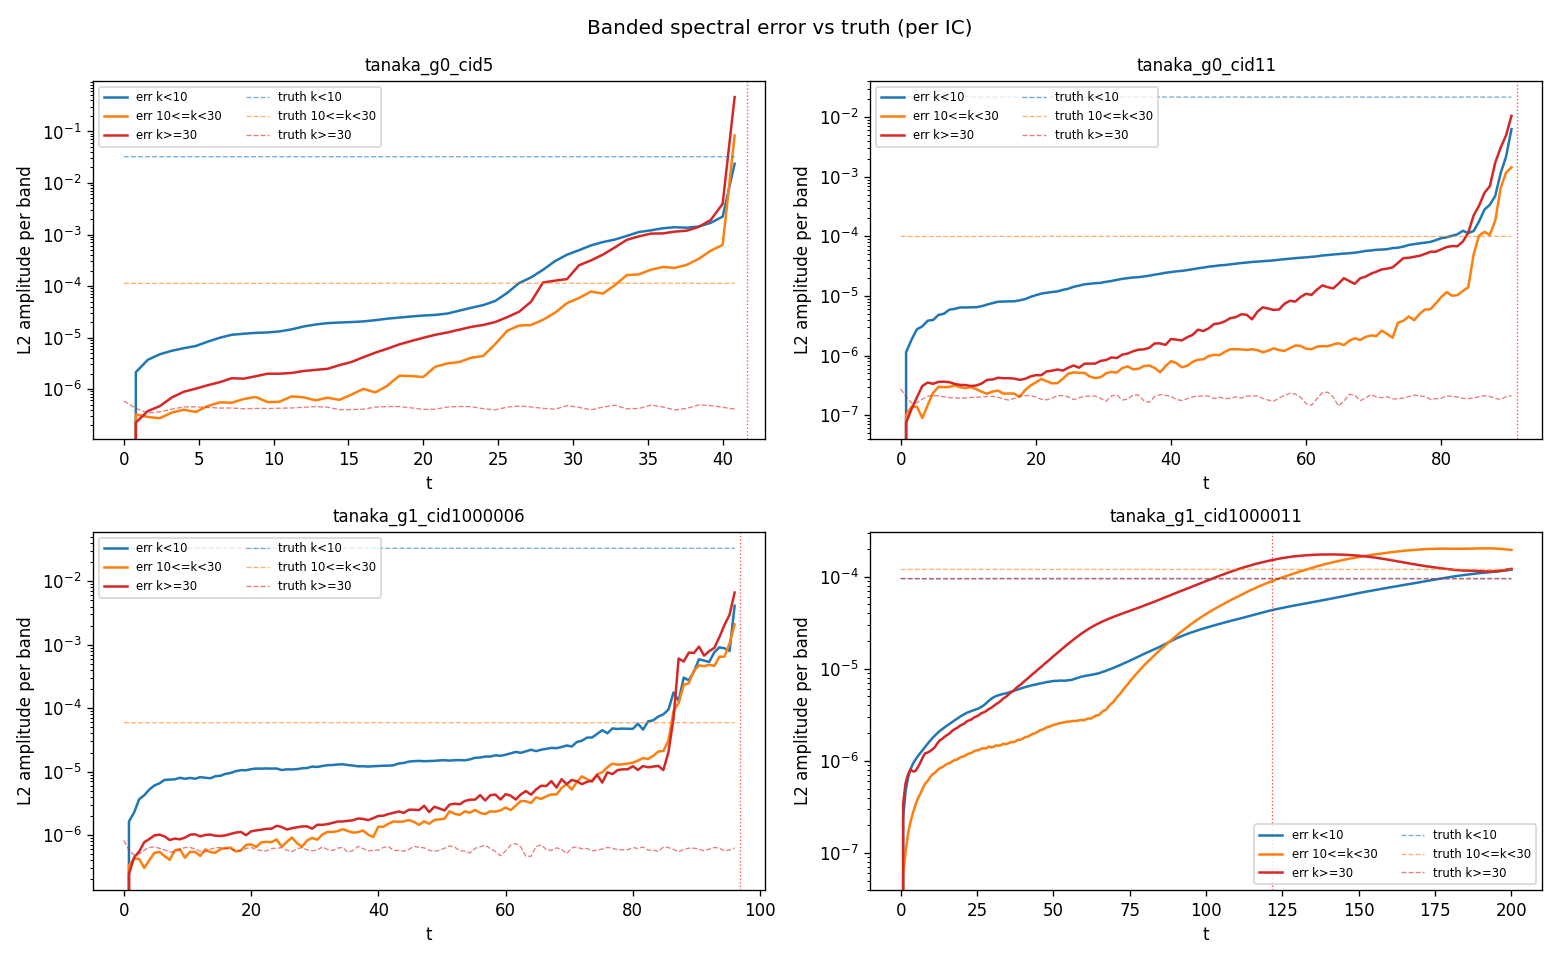
\includegraphics[width=\textwidth]{figures/tanaka_audit/banded_spectral.png}
  \caption{Fourier-band error amplitudes in representative models before C16.
  This historical figure explains why band-growth penalties and damping were
  plausible.  It is not a figure of the C21 failures described in
  Section~5.}
  \label{fig:old-band-growth}
\end{figure}

\paragraph{Inference and limitation.}
The band-growth detector was a useful warning signal, and C10's partial
improvement shows that the growing modes participate in the feedback.
However, fixed suppression either left NaNs or reduced accuracy on valid
broadband states.  These experiments therefore did not justify treating
high-frequency content itself as inadmissible.  They motivated looking for an
earlier error in the DNO map.

\subsection{Hypothesis 3: the training data were corrupt or did not constrain
the model away from reference trajectories}

\paragraph{Reason for the hypothesis.}
Pointwise supervised training evaluates $G_\theta$ on states produced by the
reference solver.  During a learned rollout, the input state is instead
produced by previous applications of $G_\theta$.  In terms of
\eqref{eq:map-split}, training can make $A_n$ small on reference states without
controlling $A_n$ on the displaced states actually visited by the model.  A
label-sign error, nonfinite row, or contaminated set of states sampled shortly
before model failure could also give a misleading gradient.

\paragraph{Tests and observations.}
A random 5,000-row audit and a separate 512-row source-stratified audit of the
base v8/v9 data found no nonfinite $\eta$, $\xi$, or $q$ values.  This is a
sampled check, not an exhaustive proof that every label is correct.  A
separate dataset harvested from model trajectories shortly before failure was
not clean reference data: 2,943 of 3,855 rows triggered the established
high-frequency/sign-change heuristic, and its balanced derivative inherited
approximately 43,000 flagged rows out of 100,000.  C13 instead generated
reference DNO labels near selected difficult Tanaka states and completed
training, but its rollout evaluation was canceled.  C13 therefore supplies no
positive or negative rollout evidence.

\paragraph{Inference and limitation.}
The audits give no support for widespread nonfinite corruption in the sampled
base data.  They do show that states harvested from a failing model should not
be treated as reference targets merely because they occur near failure.  The
broader coverage question remains open: even perfectly correct reference
snapshots need not cover every direction in which a learned rollout can leave
the reference trajectories.

\subsection{Hypothesis 4: the model value was accurate on reference states but
its derivative with respect to surface shape was wrong}

\paragraph{Reason for the hypothesis.}
For three old failing cases, the relative $q$ error obtained by evaluating the
model on the reference state was only about $1.7$--$1.9\times10^{-4}$ at the
examined frames.  This appeared too small to explain the rapid subsequent
growth by value error alone.  We therefore measured the response to a state
perturbation.  If $z^6$ is a reference state and $\delta z$ is the displacement
generated by the learned rollout, a finite secant ratio of the form
\begin{equation}
  \mathcal S
  =\frac{\norm{q_\theta(z^6+\delta z)-q_\theta(z^6)}_2}
  {\norm{\delta z}_2+\varepsilon}
  \label{eq:secant}
\end{equation}
was approximately $8.1$--$8.4$.  The change in model output induced by the
displaced state was $2.4$--$2.6\times10^4$ times the original model bias on the
reference state.  Thus small pointwise error coexisted with a much worse local
response away from the sampled trajectory.

The Hadamard identity \eqref{eq:hadamard} constrains the derivative that was
not fixed by small value error.  On three examined reference states, the learned relative
residual in \eqref{eq:hadamard} was $1.394$, $.502$, and $2.724$; the order-six
calculation gave $1.43\times10^{-5}$, $3.43\times10^{-6}$, and
$3.82\times10^{-6}$ in the same discrete test.

A Fourier perturbation supplied additional evidence.  A perturbation inserted
at input mode 117 produced an erroneous learned response at output mode 115 of
approximately $985.7$, compared with $1.47\times10^{-5}$ for the order-six
reference.  The exact $G_1$ expression \eqref{eq:g1} contains the cancellation
needed for this same-sign interaction.

\paragraph{Intervention.}
C16 changed the model and numerical implementation together:
\begin{enumerate}[leftmargin=*]
  \item $G_0+G_1$ was evaluated explicitly, with no additional cutoff;
  \item the network learned only a correction beginning at $O(\eta^2)$;
  \item tied real multipliers made the correction self-adjoint in $\xi$;
  \item randomized directions $\zeta$ were used to penalize the residual of
        \eqref{eq:hadamard}; and
  \item the quadratic part of \eqref{eq:zak-xi} was evaluated with twofold
        Fourier dealiasing.
\end{enumerate}

\paragraph{Observation.}
The clean epoch-39 C16 calculation produced no nonfinite state in 320 fixed
test rollouts without an output cap or runtime damping.  Two Tanaka cases had
finite raw elevation error above one.  By comparison, $G_0+G_1$ without the
learned correction also produced no nonfinite state in 32 Tanaka calculations,
but its median and 95th-percentile elevation errors were $.207$ and $.410$.
Thus the analytic terms alone were finite under this test but too inaccurate.

\paragraph{Inference and limitation.}
The derivative measurements directly support investigating
\eqref{eq:hadamard} and the exact $G_1$ cancellation.  The C16 result shows
that the complete bundle is compatible with finite long rollouts and useful
accuracy.  It does not establish that any one of the five changes was
individually necessary or sufficient, because they were not ablated one at a
time.  It also does not prove a zero NaN probability outside the fixed sample.


\subsection{Hypothesis 5: the base spectral loss underweighted weak but
dynamically important Fourier modes}

\paragraph{Reason for the hypothesis.}
The numerator of \eqref{eq:implemented-h1} is a single sum over modes.  A
large carrier mode can dominate this sum even when a weak sideband has a large
relative complex-coefficient error.  Benjamin--Feir evolution depends on
energy exchange among a carrier and nearby sidebands, so a loss that is small
in aggregate need not resolve that exchange.  The normalization in
\eqref{eq:mode-loss} makes a relative error in a weak active mode visible
without dividing by an arbitrarily small coefficient.

\paragraph{Intervention.}
C20 was trained from random initialization for 40 epochs.  Relative to C16,
it added both $6L_{\mathrm{mode}}$ and $10L_{\mathrm{tan}}$ as shown in
\eqref{eq:all-objectives}.  The mode term contributed approximately
2.85--2.88\% of the final training objective.  Because C20 changed two loss
terms and retrained from a new initialization, it is a test of the combined
objective rather than an ablation of $L_{\mathrm{mode}}$ alone.

\paragraph{Observation.}
All 320 trajectories in the fixed comparison suite remained finite.  Relative
to C19, the numbers of valid cases with raw terminal error above
$.25$, $.50$, $.75$, and $1$ changed from 16, 4, 2, and 0 to 10, 1, 1, and 1.
The Tanaka-g0 median and 95th percentile improved from $.07090$ and $.37295$ to
$.02281$ and $.29847$; Tanaka-g1 improved from $.12107$ and $.59621$ to
$.05212$ and $.40361$.  A fixed Benjamin--Feir case that had error $.91198$
under C19 decreased to $.36379$.  The one C20 error above one was a finite
Tanaka displacement: its raw error was $1.12696$, while its error after one
translation was $.05061$.

\paragraph{Inference and limitation.}
The result justified carrying the mode-balanced term into subsequent models:
the combined C20 retraining improved both the Tanaka and selected
Benjamin--Feir comparisons while preserving finiteness.  It does not establish
that mode balance alone caused the improvement.  The run also shows why raw
and shifted errors must both be reported: better aggregate modal accuracy did
not eliminate a slowly accumulated position error.

\subsection{Hypothesis 6: horizontal wave-speed error was weakly constrained}

\paragraph{Reason for the hypothesis.}
For a traveling wave $\eta(x,t)=\phi(x-ct)$,
\begin{equation}
  q=\eta_t=-c\eta_x.
  \label{eq:traveling-tangent}
\end{equation}
Thus the component of $q^\theta-q^*$ parallel to $\eta_x$ changes the
instantaneous translation speed.  A small persistent speed error can produce
an $O(1)$ displacement over $T=200$.

The discrete Hamiltonian \eqref{eq:discrete-H} cannot by itself detect this
error.  If $\tau_s f(x)=f(x-s)$, periodicity and translation equivariance of
the DNO give
\begin{equation}
  H(\tau_s\eta,\tau_s\xi)=H(\eta,\xi).
  \label{eq:H-translation}
\end{equation}
Therefore a prediction may have the correct Hamiltonian and the wrong
horizontal position.  This is a symmetry statement, independent of whether a
Hamiltonian penalty is used; as stated above, these runs did not use one.

For a single coherent profile, the global least-squares speed associated with
a DNO value is
\begin{equation}
  c(q;\eta)=-\frac{\inner{q}{\eta_x}}
  {\norm{\eta_x}_2^2+\varepsilon}.
  \label{eq:global-speed}
\end{equation}
For separated crests, a global inner product can cancel positive error near
one crest against negative error near another.  This motivated replacing
\eqref{eq:global-speed} by the localized construction
\eqref{eq:tangent-fields}--\eqref{eq:tangent-loss}.

\paragraph{Sequence of tests.}
\begin{enumerate}[leftmargin=*]
  \item C18 added a global translation-speed loss to a C16 checkpoint.  On the
  fixed test it improved the Tanaka-g0 median and 95th percentile to $.07963$
  and $.48205$, but did not improve Tanaka-g1: its 95th percentile increased
  from $.66002$ to $.93169$.  Framewise inspection showed cases with different
  signed errors at different crests, consistent with cancellation in
  \eqref{eq:global-speed}.

  \item C19 used the Gaussian-localized loss in \eqref{eq:tangent-loss}.  Under
  the same guarded fixed-suite protocol, the Tanaka-g0 median and 95th
  percentile became $.07090$ and $.37295$.  Several multi-crest cases improved,
  but the Benjamin--Feir-g1 and linear 95th percentiles increased.  Hence local
  translation speed was a useful target but not the complete DNO error.

  \item C21 continued from the C20 best checkpoint for one low-learning-rate
  epoch, reset Adam, and increased the coefficient of $L_{\mathrm{tan}}$ from
  10 to 100.  The weighted tangent contribution was still only $.683\%$ of the
  mean training objective.  On the fixed 64 Tanaka cases, case 27 improved
  from raw/shifted errors $1.12696/.05061$ to $.33642/.03050$.  Case 24 moved
  in the opposite direction, from $.45866/.14579$ to $.65909/.24546$.

  \item C22 began from C20, not C21, and replaced $L_{\mathrm{tan}}$ by the
  conditional growth proxy $L_\gamma$ in \eqref{eq:gamma-loss}.  The narrow
  case 27 improved further to $.18047/.02688$, but case 24 remained
  $.63952/.23662$, and the aggregate Tanaka median and 95th percentile were
  worse than C21.
\end{enumerate}

\paragraph{Inference and limitation.}
Equations \eqref{eq:traveling-tangent} and \eqref{eq:H-translation} make the
translation-speed hypothesis mathematically natural for traveling profiles,
and the experiments confirm that changing the corresponding loss moves the
phase-dominated cases.  They also show that minimizing the average projected
speed error does not bound the worst initial condition or the worst crest.
C21 and C22 are one-epoch continuations with reset optimizer state; they test
those specific update paths, not a theorem that weights 100 or 10 are optimal.
The interpretation of $L_\gamma$ is conditional on a translation-like DNO
error and does not apply to general deformation.

\subsection{Matched fixed-panel comparison of C16--C23}

Table~\ref{tab:fixed64} compares the same 32 Tanaka-g0 and 32 Tanaka-g1 case
identifiers.  This panel permits casewise comparison among checkpoints but is
not trajectory-independent of the old row-wise training split.  C19--C23 use
the same selective Tanaka runtime rule in this table; C16 does not, so the C16
row is not an exactly matched runtime-rule comparison.

\begin{table}[htbp]
\centering
\small
\begin{tabular}{lrrrrrrrr}
\toprule
& \multicolumn{4}{c}{Raw error} & \multicolumn{4}{c}{After one shift} \\
Run & Median & $q_{95}$ & Max & Count $>1$ & Median & $q_{95}$ & Max & Count $>.25$ \\
\midrule
C16 & .100430 & .602080 & 1.198696 & 2 & .025218 & .187769 & .506238 & 2 \\
C19 & .097824 & .495824 & .792011 & 0 & .013757 & .095005 & .404157 & 1 \\
C20 & .033030 & .358314 & 1.126959 & 1 & .006689 & .057147 & .394209 & 1 \\
C21 & .027887 & .344140 & .659088 & 0 & .005830 & .056214 & .341471 & 1 \\
C22 & .034449 & .376799 & .639522 & 0 & .008344 & .056436 & .361668 & 1 \\
C23 & .033732 & .367509 & 1.141937 & 1 & .006661 & .057703 & .396699 & 1 \\
\bottomrule
\end{tabular}
\caption{Matched 64-case Tanaka comparison.  C21 has the smallest median and
95th percentile in this table, but the identity of the worst case changes as
the projected losses change.}
\label{tab:fixed64}
\end{table}

\subsection{Hypothesis 7: an eight-step state loss would better represent
nonlinear error propagation}

\paragraph{Reason for the hypothesis.}
The one-state losses in Section~\ref{sec:losses} compare DNO values at a state
generated by the reference solver rather than by previous model steps.  The
desired quantity is the error after repeated
application of $\Phi_\theta$.  Equation~\eqref{eq:map-split} shows that the
effect of an early DNO error is propagated through later states.  It was
therefore reasonable to differentiate through a short segment of the same
GL2 map used in evaluation and compare the complete $(\eta,\xi)$ state rather
than only an instantaneous projection of $q$.

\paragraph{Intervention.}
C23 used the eight-step loss defined in Section~\ref{sec:losses}, over horizon
$.08$.  It was evaluated every 16 optimizer steps on four selected examples and
cycled among six source identifiers, so a particular source was used
approximately once every 96 steps.  It simultaneously set the C21 tangent
coefficient from 100 to zero.  On batches where it was evaluated, the finite-time term
contributed 2.83\% of the mean loss; after its $1/16$ duty cycle, its
approximate epoch-average contribution was $.177$\%.

\paragraph{Observation.}
Training was finite and the finite-time loss was evaluated on all 373 expected batches.  On the
fixed 64-case Tanaka panel, C23 had raw median and 95th percentile $.03373$ and
$.36751$, nearly equal to C20's $.03303$ and $.35831$ and worse than C21's
$.02789$ and $.34414$.  Case 27 returned to raw/shifted errors
$1.14194/.05014$, close to C20's $1.12696/.05061$.

\paragraph{Inference and limitation.}
This experiment did not justify replacing the dense C21 tangent term by the
tested sparse eight-step term.  It does not show that finite-time
differentiation is intrinsically ineffective.  The run changed two things at
once, used only one epoch, covered $.08$ time units out of a $T=200$ rollout,
and assigned the new term a small epoch-average weight.

\subsection{Hypothesis 8: one identifiable component of the DNO error might be
sufficient to repair the phase cases}

\paragraph{Reason for the hypothesis.}
The translation diagnostics suggested that a low-dimensional component of the
DNO error might dominate.  Before training another loss, this can be tested
within the numerical model.  At a model state $z$, define
\begin{equation}
  d(z)=q_6(z)-q_\theta(z).
  \label{eq:defect}
\end{equation}
A reference-assisted stage calculation evaluates $d(z)$ at every GL2 stage
and adds a selected component to $q_\theta(z)$.  It is not a usable surrogate,
because it calls the expensive order-six DNO.  It asks whether correcting that
selected component is sufficient in the discrete rollout.

For each active Fourier mode, the modal phase projection is
\begin{equation}
  \widehat{P_\phi d}_k
  =i\widehat\eta_k
  \frac{\operatorname{Im}(\widehat d_k\overline{\widehat\eta_k})}
       {|\widehat\eta_k|^2},
  \label{eq:modal-projection}
\end{equation}
with zero output below the target-amplitude floor.  This is the component of
$\widehat d_k$ parallel to $i\widehat\eta_k$ in the real two-dimensional
coefficient plane.  Local alternatives use the least-squares projection onto
$\eta_x$ with Gaussian widths $h$ or $4h$.  The radial complement is
$d-P_\phi d$, and the complete correction is $d$.

\paragraph{Observation.}
The same corrections were applied to fixed Tanaka cases 24 and 27:
\begin{table}[htbp]
\centering
\small
\begin{tabular}{lrrrr}
\toprule
& \multicolumn{2}{c}{Case 24} & \multicolumn{2}{c}{Case 27} \\
Stage correction & Raw & Shifted & Raw & Shifted \\
\midrule
None (C21) & .659088 & .245457 & .336422 & .030498 \\
$P_\phi d$ & .625276 & .119104 & 1.024433 & .042911 \\
Local width $h$ & .508067 & .225268 & 1.079470 & .043482 \\
Local width $4h$ & .474397 & .151743 & .134637 & .024499 \\
$d-P_\phi d$ & .137739 & .136753 & .535542 & .027532 \\
Complete $d$ & $2.25\times10^{-8}$ & $2.25\times10^{-8}$
             & $1.94\times10^{-8}$ & $1.84\times10^{-8}$ \\
\bottomrule
\end{tabular}
\caption{Reference-assisted GL2 stage corrections.  The partial correction
with the smallest final raw error is different in cases 24 and 27.}
\label{tab:stage-corrections}
\end{table}

\begin{figure}[htbp]
  \centering
  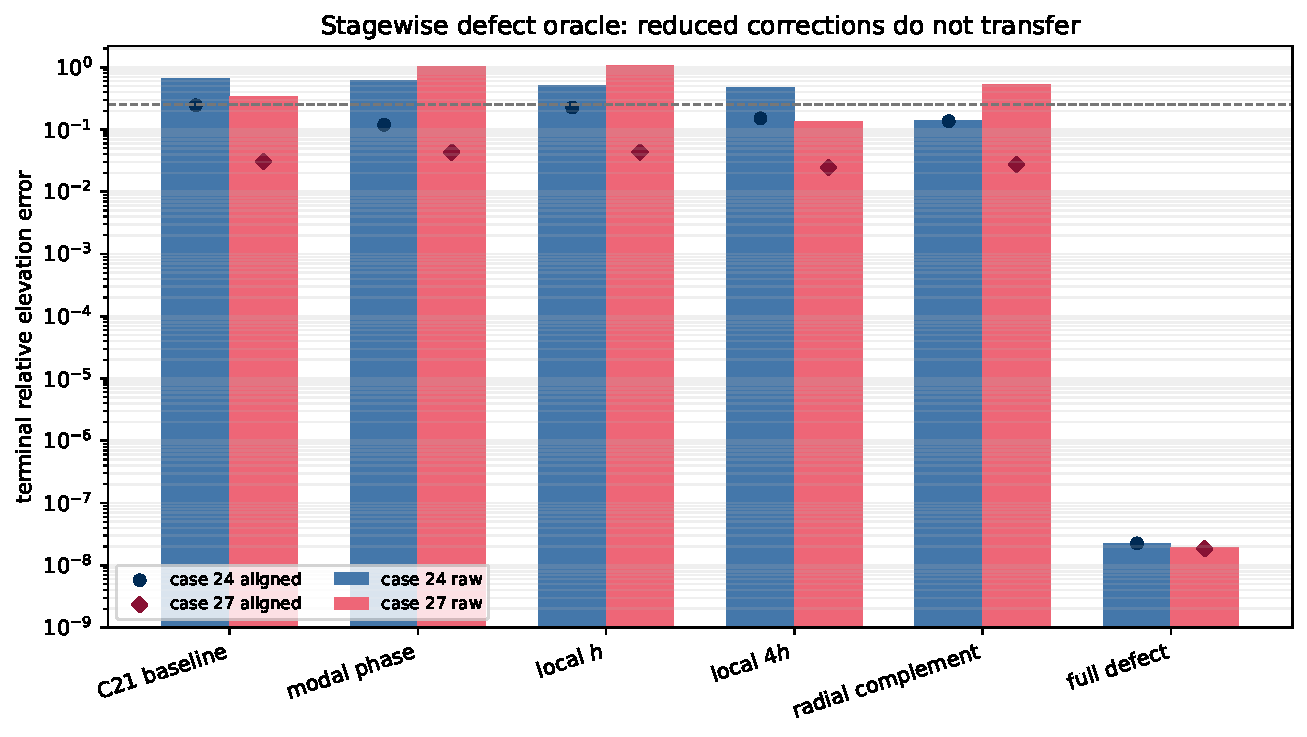
\includegraphics[width=.95\textwidth]{figures/weekly_results_20260716/c21_oracle_cross_case.pdf}
  \caption{Raw and shifted errors for the corrections in
  Table~\ref{tab:stage-corrections}.  Correcting one component can make another
  case worse.  Correcting the complete discrepancy makes the two numerical
  code paths agree to about $2\times10^{-8}$.}
  \label{fig:stage-corrections}
\end{figure}

The local-$4h$ correction gives the smallest partial-correction error for case
27 but reaches raw error $.282$ at $t=120$ before decreasing to $.135$ at
$t=200$.  Its terminal improvement therefore includes finite-time
cancellation.  The radial complement gives the smallest partial-correction
error for case 24 and worsens case 27.  The complete correction makes the
supplied DNO value equal to $q_6(z)$ at every stage; the resulting agreement is
primarily a check that the two numerical implementations are consistent.

\paragraph{Inference and limitation.}
None of the tested partial corrections improves both cases 24 and 27.  The
complete reference DNO correction reproduces the reference calculation in
both.  This does not prove that no other low-dimensional correction exists,
that GL2 is converged to the continuum equations, or that these two cases
represent all seven initial-condition distributions.  It shows only that the
specific modal, localized, and radial projections are not sufficient general
targets for these two cases.

\FloatBarrier

\section{C21 errors separated by initial-condition panel}

\begingroup
\setlength{\tabcolsep}{4pt}
\begin{longtable}{lrrrrrrrr}
\caption{C21 terminal relative elevation error separated by panel.}
\label{tab:family-errors}\\
\toprule
Panel & $n$ & \multicolumn{4}{c}{Raw error} & \multicolumn{3}{c}{After one shift} \\
& & Median & $q_{95}$ & $q_{99}$ & Max & Median & $q_{95}$ & Max \\
\midrule
\endfirsthead
\toprule
Panel & $n$ & \multicolumn{4}{c}{Raw error} & \multicolumn{3}{c}{After one shift} \\
& & Median & $q_{95}$ & $q_{99}$ & Max & Median & $q_{95}$ & Max \\
\midrule
\endhead
Tanaka g0 & 256 & .024864 & .346807 & .982779 & 1.326217 & .007272 & .077505 & .621166 \\
Tanaka g1 & 256 & .018883 & .394226 & .945614 & 1.039555 & .006300 & .067140 & .502451 \\
BF g0 & 250 & .013576 & .215374 & .351004 & .409575 & .011009 & .103352 & .223607 \\
BF g1 & 246 & .013965 & .149814 & .286310 & .327356 & .010258 & .078148 & .279071 \\
BF modal & 244 & .015984 & .272954 & .607009 & 1.103567 & .011789 & .106436 & .842246 \\
Linear & 241 & .001629 & .080299 & .485923 & .841318 & .001354 & .051359 & .634983 \\
Random sea, deep & 256 & .001482 & .014397 & .026108 & .036360 & .001482 & .014386 & .036356 \\
Random sea, finite depth & 254 & .002353 & .032527 & .078271 & .133546 & .002352 & .032525 & .133498 \\
Stokes, deep & 256 & .000342 & .001384 & .002354 & .008859 & .000082 & .000429 & .000753 \\
Stokes, finite depth & 249 & .001933 & .023278 & .161884 & .546789 & .000405 & .003323 & .076945 \\
\bottomrule
\end{longtable}
\endgroup

The large errors are not distributed uniformly across the panels.  Tanaka g0
contains 17 cases above .25 and 3 above 1.  Tanaka g1 contains 26 cases above
.25 and 2 above 1.  BF modal contains 15 cases above .25 and 1 above 1.  The
two random-sea panels and the deep Stokes panel contain no case above .25.
Because each panel has at most 256 valid cases, the empirical 95th percentile
is determined by only about thirteen observations above it.  These results
are therefore useful empirical error distributions, not estimates of
arbitrarily rare-event probabilities.

\section{What causes the six errors above one?}

This section uses three separate diagnostics.  First, the translation error
\eqref{eq:shift-error} asks whether one final spatial shift explains the
elevation discrepancy.  Second, Fourier phase rates test whether the observed
shift is accumulated through the kinematic equation $\eta_t=q$.  Third, a
same-state decomposition of $q$ distinguishes the learned operator error from
the response of the numerical reference to an already incorrect state.

\subsection{Five Tanaka cases: horizontal displacement accumulates over time}

Table~\ref{tab:tanaka-six} lists the five Tanaka cases with raw error above
one.  A single translation removes at least 98.14\% of the squared terminal
elevation error in every case.  In four cases it removes more than 99.89\%.
This establishes that horizontal position accounts for most of the terminal
$\ell^2$ discrepancy.  It does not, by itself, prove that the dynamical error
at all earlier times lies in a single translation eigenvector.

\begin{table}[htbp]
\centering
\small
\begin{tabular}{llrrrr}
\toprule
Panel & Index & Raw error & Shifted error & Shift (grid cells) & $r_{\rm shift}$ \\
\midrule
Tanaka g0 & 91  & 1.326217 & .036765 & 15.736 & 99.923\% \\
Tanaka g0 & 186 & 1.091708 & .034695 & 10.898 & 99.899\% \\
Tanaka g0 & 224 & 1.128034 & .154012 & 9.065  & 98.136\% \\
Tanaka g1 & 88  & 1.026072 & .025568 & 7.159  & 99.938\% \\
Tanaka g1 & 202 & 1.039555 & .021458 & 7.725  & 99.957\% \\
\bottomrule
\end{tabular}
\caption{The five Tanaka cases with raw terminal error above one.  The last
column is defined in \eqref{eq:rshift}.}
\label{tab:tanaka-six}
\end{table}

\begin{figure}[htbp]
  \centering
  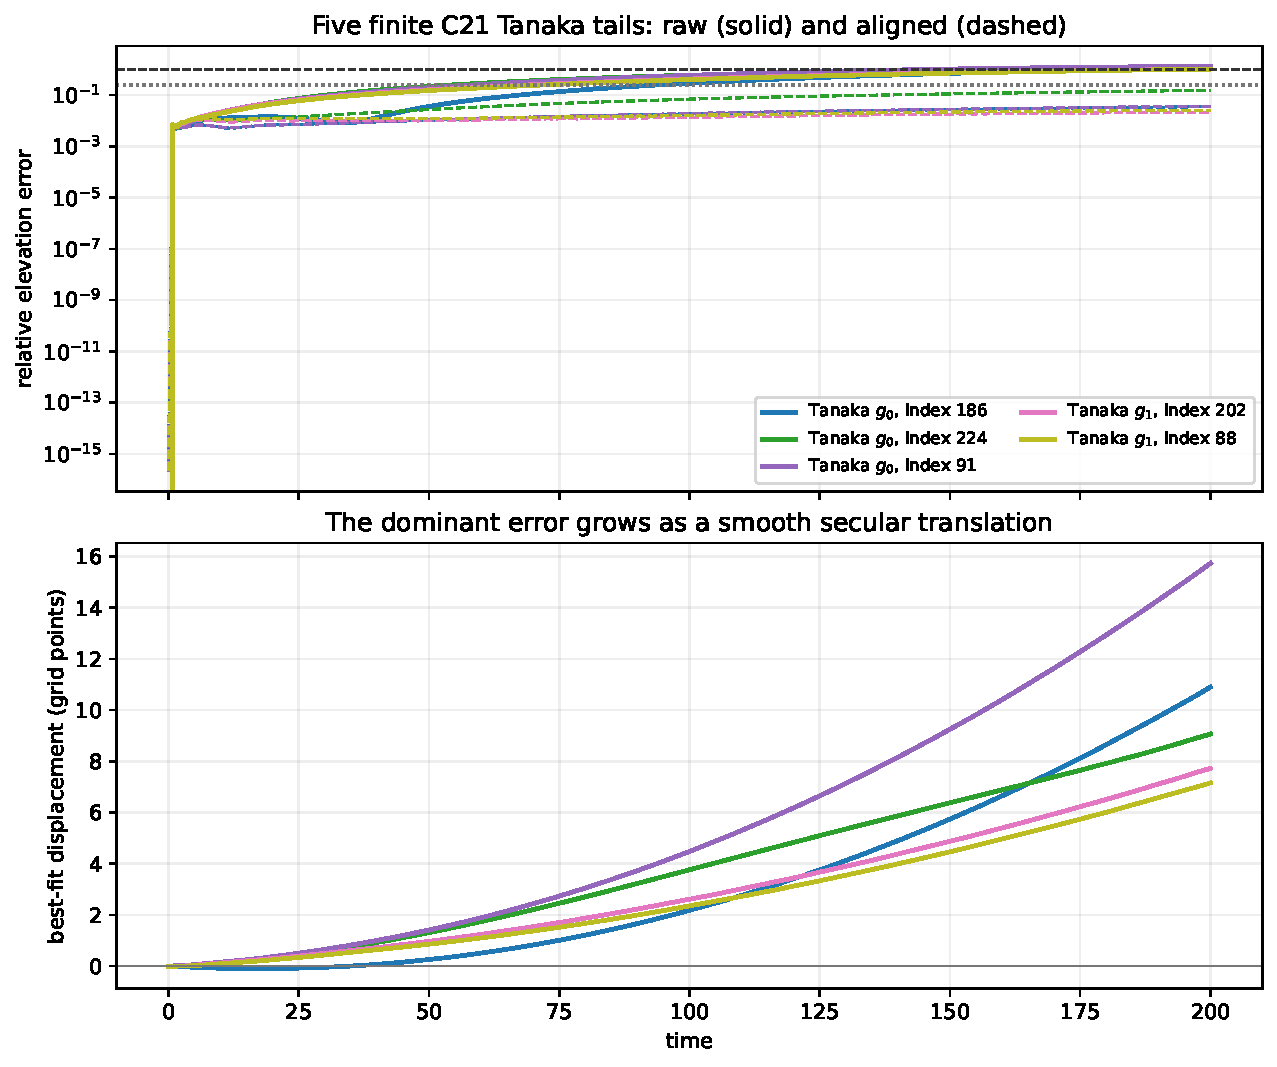
\includegraphics[width=.92\textwidth]{figures/weekly_results_20260716/c21_worst_tanaka_error_growth.pdf}
  \caption{Raw elevation error, error after the best translation at each saved
  time, and the corresponding translation for the five cases in
  Table~\ref{tab:tanaka-six}.  The translations grow over the full interval
  rather than appearing in one final step.}
  \label{fig:tanaka-growth}
\end{figure}

\begin{figure}[htbp]
  \centering
  \begin{subfigure}[t]{.49\textwidth}
    \centering
    
\includegraphics[width=\textwidth]{\detokenize{figures/weekly_results_20260716/failure_frames/tanaka_g0_idx=91_case90000091_h0.018_final.png}}
    \caption{Index 91: raw error 1.326; shifted error .0368.}
  \end{subfigure}
  \hfill
  \begin{subfigure}[t]{.49\textwidth}
    \centering
    
\includegraphics[width=\textwidth]{\detokenize{figures/weekly_results_20260716/failure_frames/tanaka_g0_idx=224_case90000224_h0.014_final.png}}
    \caption{Index 224: raw error 1.128; shifted error .154.}
  \end{subfigure}
  \caption{Final order-six elevation (black) and C21 elevation (red dashed).
  Index 91 is nearly a rigid translation.  Index 224 also has a visible shape
  or relative-crest-position error after the best global shift.}
  \label{fig:tanaka-frames}
\end{figure}

\subsubsection{Why an error in \texorpdfstring{$q$}{q} produces a phase error}

For a nonzero Fourier coefficient write
\begin{equation}
  \widehat\eta_k(t)=a_k(t)e^{i\phi_k(t)},
  \qquad a_k(t)>0.
\end{equation}
Since $\partial_t\widehat\eta_k=\widehat q_k$, division by
$\widehat\eta_k$ gives
\begin{equation}
  \frac{\widehat q_k}{\widehat\eta_k}
  =\frac{\dot a_k}{a_k}+i\dot\phi_k,
  \qquad
  \dot\phi_k=\operatorname{Im}
  \left(\frac{\widehat q_k}{\widehat\eta_k}\right).
  \label{eq:phase-rate}
\end{equation}
Equation~\eqref{eq:phase-rate} is an identity whenever
$\widehat\eta_k\ne0$.  In the numerical audit it is applied only to retained
modes whose amplitudes exceed the stated activity floor.

For modes 1--8 in the five cases of Table~\ref{tab:tanaka-six}, integrating
the difference between C21 and reference phase rates reconstructs the measured
terminal phase difference to within $3.8\times10^{-4}$ radians.  Independently,
for modes 1--4, numerical integration of $q=\eta_t$ reconstructs the observed
change in $\widehat\eta_k$ with 1.0--1.7\% relative discrepancy.  These checks
support the following limited conclusion: the saved $q$ discrepancy is
consistent with the observed gradual phase accumulation.  They do not prove
that the continuum solution has the same phase, because the comparison is to
the order-six numerical reference.

\subsubsection{Learned DNO error versus propagation of existing state error}

At any state $z=(\eta,\xi)$ define
\begin{equation}
  q_\theta(z)=G_\theta(\eta)\xi,
  \qquad q_6(z)=G_6(\eta)\xi.
\end{equation}
At the model and reference states, direct addition and subtraction gives
\begin{equation}
\begin{split}
 q_\theta(z_\theta)-q_6(z_6)
 ={}&\underbrace{q_\theta(z_\theta)-q_6(z_\theta)}_{
       \text{DNO approximation error at the model state}}\\
 &+\underbrace{q_6(z_\theta)-q_6(z_6)}_{
       \text{change in the reference DNO caused by state separation}}.
\end{split}
\label{eq:q-split}
\end{equation}
This is the continuous-stage analogue of \eqref{eq:map-split}.  At the final
saved time in the five Tanaka cases, the first term in \eqref{eq:q-split} has
relative norm approximately .38--1.19\%, whereas the second has relative norm
3.14--11.75\%.  This does not absolve the learned DNO: the second term is zero
when the states agree and grows only after earlier errors have separated the
trajectories.  It does show why reducing only the instantaneous DNO error on
reference-supplied states may not proportionally reduce the final displacement.

\subsection{One Benjamin--Feir case: a single translation is insufficient}

BF-modal index 22 has raw error $1.10357$ and shifted error $0.84225$.  From
\eqref{eq:rshift}, one translation removes only 41.75\% of the squared error.
At Fourier modes 17, 20, and 23, the final predicted-to-reference amplitude
ratios are respectively $1.495$, $.305$, and $.968$.  Shifts inferred from
the individual phase differences are $-.00699$, $+.07027$, and $-.06199$.
Their differing signs show that no single translation can align all three
modes.  The calculation remains finite; the error is in the relative
amplitudes and phases of the carrier and neighboring modes.

\begin{figure}[htbp]
  \centering
  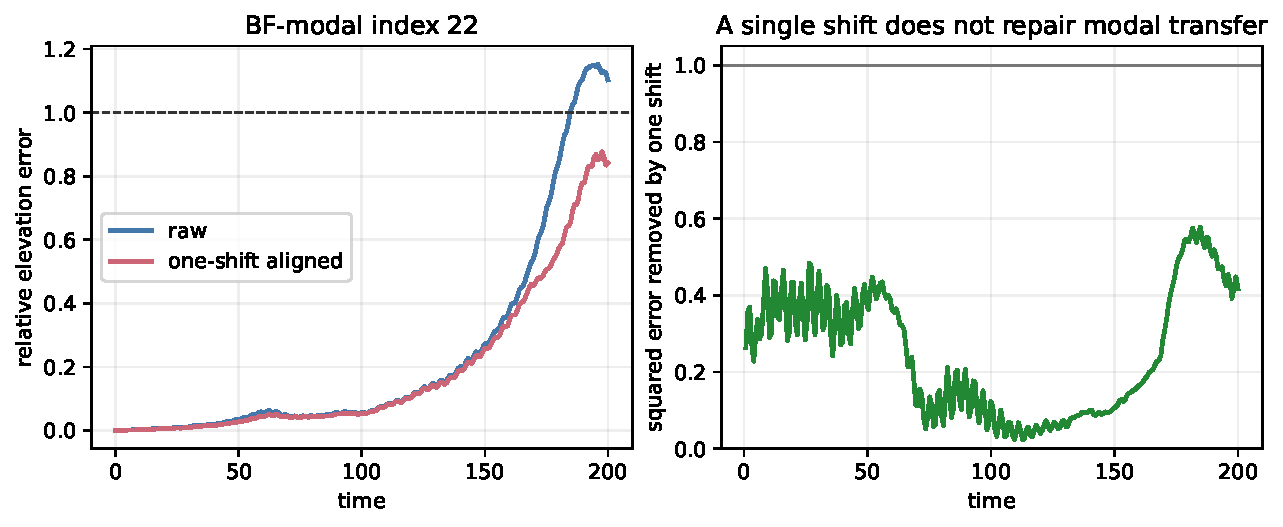
\includegraphics[width=.9\textwidth]{figures/weekly_results_20260716/c21_worst_bf_modal_error_growth.pdf}
  \caption{Raw error, error after one horizontal translation, and the fraction
  of squared error removed for BF-modal index 22.  At the final time, the best
  translation leaves relative elevation error .842.}
  \label{fig:bf-growth}
\end{figure}

\begin{figure}[htbp]
  \centering
  
\includegraphics[width=.82\textwidth]{\detokenize{figures/weekly_results_20260716/failure_frames/bf_modal_idx=22_case94000022_h2.876_final.png}}
  \caption{Final order-six and C21 profiles for BF-modal index 22, together
  with the saved errors in $\eta$, $\xi$, and $q$.  The discrepancy cannot be
  removed by translating the complete profile.}
  \label{fig:bf-frame}
\end{figure}

\FloatBarrier

\FinalSections
\end{document}
